\begin{block}{Introduction}
    \textbf{Overview.\space}The project is based on a cross-platform application framework that encourages students to exchange their books and ideas on an online platform.\\
    \textbf{Motivation.\space} This project aimed to solve two major problems:
    \begin{itemize}
        \item Allow students to meet more friends through the use of social media application. \cite{covid19:2022jd,Parlak:2012qr}
        \item Address the problem of wasted textbooks by encouraging them to exchange the used books.
    \end{itemize}
    \textbf{Technical Background.\space}The application is targeted to deploy on iOS and Android.
    \begin{itemize}
        \item Frontend: Flutter framework + Dart language \cite{Flutter:Documentation}
            \begin{itemize}
                \item[--] Only a single codebase is used
                \item[--] Code is rendered as widgets in the element tree to represent the current state of user interface
                \item[--] The rendering tree is then used to generate a platform-agnostic Skia canvas
                \item[--] GPU renders the UI to the screen to achieve cross-platform effect
            \end{itemize}
            \begin{figure}
                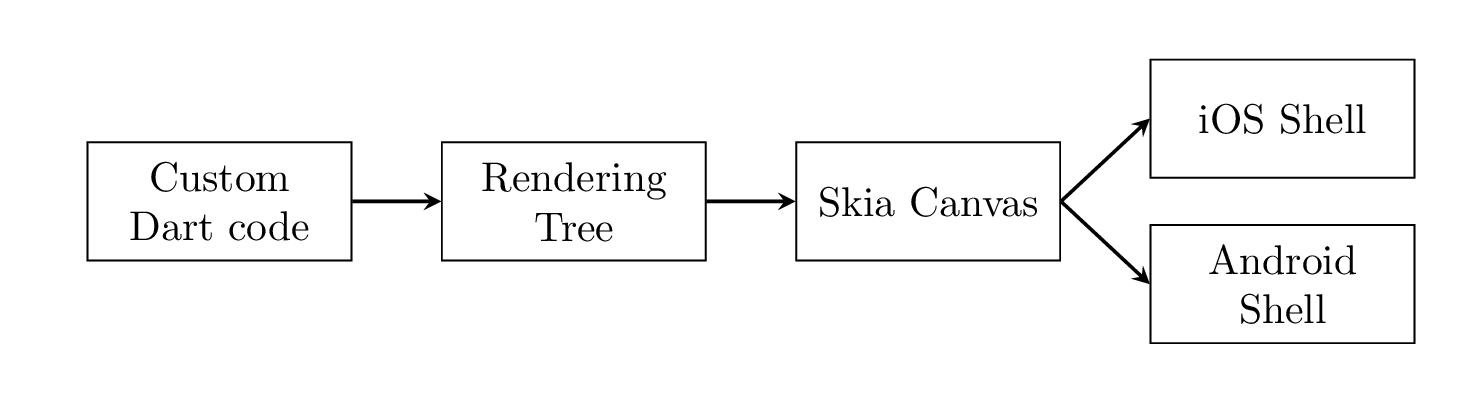
\includegraphics[width=\linewidth]{rendering.png}
                \caption{Flutter rendering process}
            \end{figure}
        \vspace{-2.3cm}
        \item Backend: Node.js server to create various APIs
        \item Database: MongoDB to create non-relational documents \cite{MongoDB:Documentation}
        \begin{figure}
            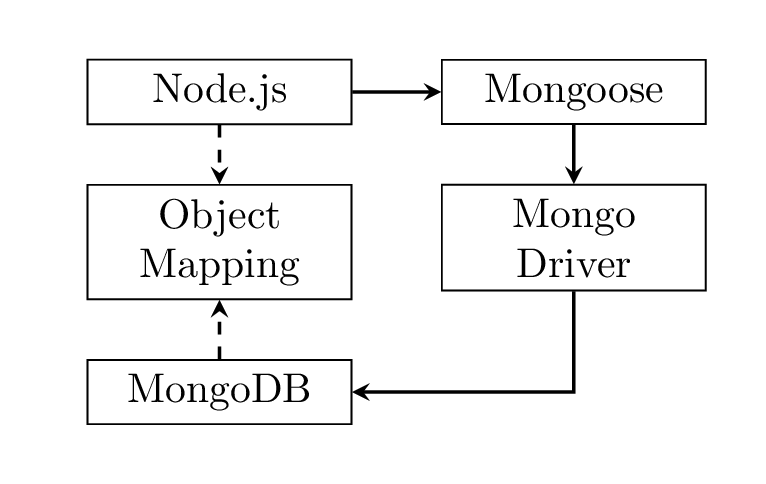
\includegraphics[width=0.8\linewidth]{backend.png}
            \caption{Nodejs and MongoDB relations}
        \end{figure}
        \vspace{-2.3cm}
        Node.js uses the Mongoose package as the driver to communicate with MongoDB and perform various actions. The Schema and models are defined using Mongoose API and send the queries back to the server in JSON-format.
    \end{itemize}
\end{block}